\section{実験原理}\label{pi2flipper_sec}
\subsection{概要}
\begin{figure}[h]
\begin{center}
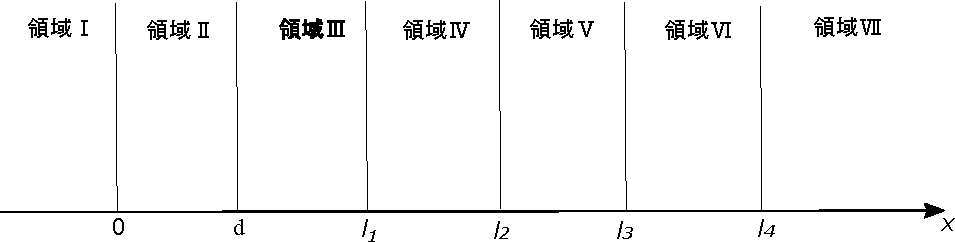
\includegraphics[width=13cm]{pi2flipper/zenntaizu.pdf}
\caption{実験装置の概要}
\end{center}
\end{figure}
今回の実験装置の概要を図に示す。ビームは領域Ⅰから入射し、各領域を通過して、領域Ⅶにある検出器で検出される。領域Ⅰから領域Ⅶにかけて、全体に$z方向の一様磁場B_{z}$がかかっている。領域Ⅱと領域Ⅵには$\pi/2フリッパー$があり、$x方向の振動磁場2B_{r}\cos(\omega_{s}t)$がかかっている。領域Ⅳには位相シフタコイルがあり、$z方向に磁場B+B_{z}$がかかっている。
ここでは、領域Ⅰから、
\begin{align}
{\psi}_{Ⅰ}(x,t)=
\begin{pmatrix}
1 \\
0
\end{pmatrix}
e^{ik_{0}^{+}x}e^{-i\omega_{0}t}
\end{align}
のような波動関数で表される粒子が、領域Ⅶでどのような状態になるのかを考え、領域Ⅶで干渉が現れることを見る。磁場によるエネルギーが入射波のエネルギーよりも十分に小さいと仮定する。つまり、
\begin{align}
\omega_{0} \gg |{\mu}|B_{r},  |{\mu}|B_{z},  |{\mu}|B
\end{align}
と仮定する。このとき、のちにわかるように、各領域の境界における反射波は無視できる。
\subsection{詳細な計算}
\paragraph{領域Ⅱにおけるスピンのフリップ}
領域Ⅱにおける磁場は
\begin{align}
\bm{B}=2B_{r}\cos(\omega_{s}t)\bm{\hat{x}}+B_{z}\bm{\hat{z}}
\end{align}
であるが、$B_{z} \gg B_{r}$の時は、のちに述べる理由により、$2B_{r}\cos(\omega_{s}t)\bm{\hat{x}} \to  B_{r}\cos(\omega_{s}t)\bm{\hat{x}}+B_{r}\sin(\omega_{s}t)\bm{\hat{y}}$とできる。ゆえに、領域Ⅱにおける磁場は
\begin{align}
\bm{B}=B_{r}\cos(\omega_{s}t)\bm{\hat{x}}+B_{r}\sin(\omega_{s}t)\bm{\hat{y}}+B_{z}\bm{\hat{z}}
\end{align}
であるとする。
\begin{align}
\omega_{r}=|{\mu}|B_{r}
\end{align}
\begin{align}
\omega_{z}=|{\mu}|B_{z}
\end{align}
とする。この時、領域Ⅱにおけるシュレディンガー方程式は
\begin{align}
i\frac{\partial {\psi}_{Ⅱ}(x,t)}{\partial t}=\left(-\frac{1}{2m}\frac{\partial^2}{\partial x^2}+\omega_{r}\cos(\omega_{s}t){\sigma}_{x}+\omega_{r}\sin(\omega_{s}t){\sigma}_{y}+\omega_{z}{\sigma}_{z}\right){\psi}_{Ⅱ}(x,t)
\end{align}
と書ける。ここで、
\begin{align}
\omega_{r}\cos(\omega_{s}t){\sigma}_{x}+\omega_{r}\sin(\omega_{s}t){\sigma}_{y}+\omega_{z}{\sigma}_{z}=
\begin{pmatrix}
\omega_{z} &\omega_{r}e^{-i\omega_{s}t} \\
\omega_{r}e^{i\omega_{s}t} &-\omega_{z}
\end{pmatrix}
\end{align}
$と書ける。角速度\omega_{s}でz軸の周りに回転するユニタリー変換$
\begin{align}
U_{T}=\exp(i\omega_{s}t{\sigma}_{z}/2)=
\begin{pmatrix}
e^{i\omega_{s}t/2} &0 \\
0 &e^{-i\omega_{s}t/2}
\end{pmatrix}
\end{align}
をもちいて
\begin{align}
U_{T}\begin{pmatrix}
\omega_{z} &\omega_{r}e^{-i\omega_{s}t} \\
\omega_{r}e^{i\omega_{s}t} &-\omega_{z}
\end{pmatrix}U_{T}^{\dagger}=
\begin{pmatrix}
\omega_{z} &\omega_{r} \\
\omega_{r} &-\omega_{z}
\end{pmatrix}
\end{align}
が成り立つ。
\begin{align}
{\psi}_{R}(x,t)=U_{T}{\psi}(x,t)
\end{align}
$とすると{\psi}_{R}(x,t)の満たすシュレディンガー方程式は$
\begin{align}
i\frac{\partial {\psi}_{R}(x,t)}{\partial t}=\left(-\frac{1}{2m}\frac{\partial^2}{\partial x^2}+\omega_{r}{\sigma}_{x}+\left(\omega_{z}-\frac{1}{2}\omega_{s}\right){\sigma}_{z}\right){\psi}_{R}(x,t)
\end{align}
となる。いま、共鳴条件
\begin{align}
{\epsilon}=\frac{1}{2}\omega_{s}-\omega_{z}=0\label{pi2flipper_resonance}
\end{align}
が成り立っているとする。この時、シュレディンガー方程式は
\begin{align}
i\frac{\partial {\psi}_{R}(x,t)}{\partial t}=\left(-\frac{1}{2m}\frac{\partial^2}{\partial x^2}+\omega_{r}{\sigma}_{x}\right){\psi}_{R}(x,t)
\end{align}
いま、
\begin{align}
U_{D}=\exp(i{\pi}{\sigma}_{y}/4)=
\begin{pmatrix}
1/\sqrt{2} &1/\sqrt{2} \\
-1/\sqrt{2} &1/\sqrt{2}
\end{pmatrix}
\end{align}
というユニタリー変換を用いると、
\begin{align}
U_{D}{\sigma}_{x}U_{D}^{\dagger}={\sigma}_{z}
\end{align}
が成り立つ。
\begin{align}
{\psi}_{D}(x,t)=U_{D}{\psi}_{R}(x,t)
\end{align}
$とすると、{\psi}_{D}(x,t)の満たすシュレーディンガー方程式は$
\begin{align}
i\frac{\partial {\psi}_{D}(x,t)}{\partial t}=\left(-\frac{1}{2m}\frac{\partial^2}{\partial x^2}+\omega_{r}{\sigma}_{z}\right){\psi}_{D}(x,t)
\end{align}
$この方程式の解のうち、エネルギー固有値がE_{n}=\omega_{n}であるものは$
\begin{align}
{\psi}_{D}(x,t) =
\begin{pmatrix}
A_{n}^{+}e^{ik_{n}^{+}x}+B_{n}^{+}e^{-ik_{n}^{+}x}  \\
A_{n}^{-}e^{ik_{n}^{-}x}+B_{n}^{-}e^{-ik_{n}^{-}x}
\end{pmatrix}
e^{-i\omega_{n}t}
\end{align}
ここで、
\begin{align}
\frac{{k_{n}^{\pm}}^2}{2m}{\pm}\omega_{r}=E_{n}
\end{align}
が成り立つ。ゆえに、領域Ⅱにおける波動関数は
\begin{align}
{\psi}_{Ⅱ}(x,t)=U_{T}^{\dagger}U_{D}^{\dagger}{\psi}_{D}(x,t)=\frac{1}{\sqrt{2}}
\begin{pmatrix}
\left((A_{n}^{+}e^{ik_{n}^{+}x}+B_{n}^{+}e^{-ik_{n}^{+}x})-(A_{n}^{-}e^{ik_{n}^{-}x}+B_{n}^{-}e^{-ik_{n}^{-}x})\right)e^{-i(\omega_{n}+\omega_{z})t} \\
\left((A_{n}^{+}e^{ik_{n}^{+}x}+B_{n}^{+}e^{-ik_{n}^{+}x})+(A_{n}^{-}e^{ik_{n}^{-}x}+B_{n}^{-}e^{-ik_{n}^{-}x})\right)e^{-i(\omega_{n}-\omega_{z})t}
\end{pmatrix}
\end{align}
$ここで、1/{\sqrt{2}}A_{n}^{\pm}, 1/{\sqrt{2}}B_{n}^{\pm}をA_{n}^{\pm}, B_{n}^{\pm}と取り直すと、$
\begin{align}
{\psi}_{Ⅱ}(x,t)=U_{T}^{\dagger}U_{D}^{\dagger}{\psi}_{D}(x,t)=
\begin{pmatrix}
\left((A_{n}^{+}e^{ik_{n}^{+}x}+B_{n}^{+}e^{-ik_{n}^{+}x})-(A_{n}^{-}e^{ik_{n}^{-}x}+B_{n}^{-}e^{-ik_{n}^{-}x})\right)e^{-i(\omega_{n}+\omega_{z})t} \\
\left((A_{n}^{+}e^{ik_{n}^{+}x}+B_{n}^{+}e^{-ik_{n}^{+}x})+(A_{n}^{-}e^{ik_{n}^{-}x}+B_{n}^{-}e^{-ik_{n}^{-}x})\right)e^{-i(\omega_{n}-\omega_{z})t}
\end{pmatrix}
\end{align}
いま、入射波を
\begin{align}
\begin{pmatrix}
I_{0}^{+} \\
0
\end{pmatrix}
e^{ik_{0}^{+}x}e^{-i\omega_{0}t}
\end{align}
とする。ここで、
\begin{align}
\omega_{1}=\omega_{0}-\omega_{z}
\end{align}
$とすると、x=0における接続より、領域Ⅱにおいてn=1のもの以外は0になる。この時、スピン下成分のエネルギーは、$
\begin{align}
\omega_{1}-\omega_{z}=\omega_{0}-2\omega_{z}
\end{align}
$である。ゆえに、x=0における反射を考慮すると、領域Ⅰにおける波動関数は$
\begin{align}
{\psi}_{Ⅰ}(x,t)=
\begin{pmatrix}
(I_{0}^{+}e^{ik_{0}^{+}x}+R_{0}^{+}e^{-ik_{0}^{+}x})e^{-i\omega_{0}t} \\
R_{2}^{-}e^{-ik_{2}^{-}x}e^{-i(\omega_{0}-2\omega_{z})t}
\end{pmatrix}
\end{align}
のようにかける。ここで、
\begin{align}
&\frac{(k_{0}^+)^{2}}{2m}+\omega_{z}=\omega_{0} \\
&\frac{(k_{2}^-)^{2}}{2m}-\omega_{z}=\omega_{0}-2\omega_{z}
\end{align}
$が成り立つ。x=0における接続により、$
\begin{align}
&(A_{1}^{+}+B_{1}^{+})-(A_{1}^{-}+B_{1}^{-})=I_{0}^{+}+R_{0}^{+} \\
&k_{1}^{+}(A_{1}^{+}-B_{1}^{+})-k_{1}^{-}(A_{1}^{-}-B_{1}^{-})=k_{0}^{+}I_{0}^{+}-k_{0}^{+}R_{0}^{+} \\
&(A_{1}^{+}+B_{1}^{+})+(A_{1}^{-}+B_{1}^{-})=R_{2}^{-} \\
&k_{1}^{+}(A_{1}^{+}-B_{1}^{+})+k_{1}^{-}(A_{1}^{-}-B_{1}^{-})=-k_{2}^{-}R_{2}^{-}
\end{align}
が成り立つ。以下、
\begin{align}
\omega_{0} \gg |{\mu}|B_{r},  |{\mu}|B_{z},  |{\mu}|B
\end{align}
$に従って、k_{1}^{+}などをすべてk_{0}で近似する。しかし、指数の肩に現れているものはk_{0}からのずれが重要になるので、そのままにしておく。この近似が反射波を無視することに対応する。$
\begin{align}
&A_{1}^{+}+B_{1}^{+}-A_{1}^{-}-B_{1}^{-}=I_{0}^{+}+R_{0}^{+} \\
&A_{1}^{+}-B_{1}^{+}-A_{1}^{-}+B_{1}^{-}=I_{0}^{+}-R_{0}^{+} \\
&A_{1}^{+}+B_{1}^{+}+A_{1}^{-}+B_{1}^{-}=R_{2}^{-} \\
&A_{1}^{+}-B_{1}^{+}+A_{1}^{-}-B_{1}^{-}=-R_{2}^{-}
\end{align}
ゆえに
\begin{align}
&A_{1}^{+}-A_{1}^{-}=I_{0}^{+} \\
&B_{1}^{+}-B_{1}^{-}=R_{0}^{+} \\
&A_{1}^{+}+A_{1}^{-}=0 \\
&B_{1}^{+}+B_{1}^{-}=R_{2}^{-}
\end{align}
$透過波、すなわち領域Ⅲにおける波動関数のうち、エネルギー固有値がE_{n}であるものは以下のようなものである。$
\begin{align}
{\psi}_{Ⅲ}(x,t)=
\begin{pmatrix}
C_{n}^{+}e^{iK_{n}^{+}x}e^{-i\omega_{n}t} \\
C_{n}^{-}e^{iK_{n}^{-}x}e^{-i\omega_{n}t} 
\end{pmatrix}
\end{align}
ここで、
\begin{align}
\omega_{2}=\omega_{0}-2\omega_{z}
\end{align}
$とすると、x=x_{1}における接続より、スピン上成分についてはn=0のみが残り、スピン下成分についてはn=2のみが残る。$
\begin{align}
{\psi}_{Ⅲ}(x,t)=
\begin{pmatrix}
C_{0}^{+}e^{iK_{0}^{+}x}e^{-i\omega_{0}t} \\
C_{2}^{-}e^{iK_{2}^{-}x}e^{-i\omega_{2}t} 
\end{pmatrix}
\end{align}
$x=x_{1}における接続より、$
\begin{align}
&C_{0}^{+}e^{iK_{0}^{+}x_{1}}=(A_{1}^{+}e^{ik_{1}^{+}x_{1}}+B_{1}^{+}e^{-ik_{1}^{+}x_{1}})-(A_{1}^{-}e^{ik_{1}^{-}x_{1}}+B_{1}^{-}e^{-ik_{1}^{-}x_{1}}) \\
&K_{0}^{+}C_{0}^{+}e^{iK_{0}^{+}x_{1}}=k_{0}^{+}(A_{1}^{+}e^{ik_{1}^{+}x_{1}}-B_{1}^{+}e^{-ik_{1}^{+}x_{1}})-k_{0}^{-}(A_{1}^{-}e^{ik_{1}^{-}x_{1}}-B_{1}^{-}e^{-ik_{1}^{-}x_{1}}) \\
&C_{2}^{-}e^{iK_{2}^{-}x_{1}}=(A_{1}^{+}e^{ik_{1}^{+}x_{1}}+B_{1}^{+}e^{-ik_{1}^{+}x_{1}})+(A_{1}^{-}e^{ik_{1}^{-}x_{1}}+B_{1}^{-}e^{-ik_{1}^{-}x_{1}}) \\
&K_{2}^{-}C_{2}^{-}e^{iK_{2}^{-}x_{1}}=k_{0}^{+}(A_{1}^{+}e^{ik_{1}^{+}x_{1}}-B_{1}^{+}e^{-ik_{1}^{+}x_{1}})+k_{0}^{-}(A_{1}^{-}e^{ik_{1}^{-}x_{1}}-B_{1}^{-}e^{-ik_{1}^{-}x_{1}}) 
\end{align}
先ほどと同じように近似して
\begin{align}
&C_{0}^{+}e^{iK_{0}^{+}x_{1}}=A_{1}^{+}e^{ik_{1}^{+}x_{1}}+B_{1}^{+}e^{-ik_{1}^{+}x_{1}}-A_{1}^{-}e^{ik_{1}^{-}x_{1}}-B_{1}^{-}e^{-ik_{1}^{-}x_{1}} \\
&C_{0}^{+}e^{iK_{0}^{+}x_{1}}=A_{1}^{+}e^{ik_{1}^{+}x_{1}}-B_{1}^{+}e^{-ik_{1}^{+}x_{1}}-A_{1}^{-}e^{ik_{1}^{-}x_{1}}+B_{1}^{-}e^{-ik_{1}^{-}x_{1}} \\
&C_{2}^{-}e^{iK_{2}^{-}x_{1}}=A_{1}^{+}e^{ik_{1}^{+}x_{1}}+B_{1}^{+}e^{-ik_{1}^{+}x_{1}}+A_{1}^{-}e^{ik_{1}^{-}x_{1}}+B_{1}^{-}e^{-ik_{1}^{-}x_{1}} \\
&C_{2}^{-}e^{iK_{2}^{-}x_{1}}=A_{1}^{+}e^{ik_{1}^{+}x_{1}}-B_{1}^{+}e^{-ik_{1}^{+}x_{1}}+A_{1}^{-}e^{ik_{1}^{-}x_{1}}-B_{1}^{-}e^{-ik_{1}^{-}x_{1}} \\
\end{align}
ゆえに
\begin{align}
&C_{0}^{+}e^{iK_{0}^{+}x_{1}}=A_{1}^{+}e^{ik_{1}^{+}x_{1}}-A_{1}^{-}e^{ik_{1}^{-}x_{1}} \\
&0=B_{1}^{+}e^{-ik_{1}^{+}x_{1}}-B_{1}^{-}e^{-ik_{1}^{-}x_{1}} \\
&C_{2}^{-}e^{iK_{2}^{-}x_{1}}=A_{1}^{+}e^{ik_{1}^{+}x_{1}}+A_{1}^{-}e^{ik_{1}^{-}x_{1}} \\
&0=B_{1}^{+}e^{-ik_{1}^{+}x_{1}}+B_{1}^{-}e^{-ik_{1}^{-}x_{1}} \\
\end{align}
よって、
\begin{align}
&B_{1}^{+}=B_{1}^{-}=0 \\
\end{align}
ゆえに、
\begin{align}
&R_{0}^{+}=B_{1}^{+}-B_{1}^{-}=0 \\
&R_{2}^{-}=B_{1}^{+}+B_{1}^{-}=0
\end{align}
$よって、この近似の下では、反射波は無視できる。入射波の振幅I_{0}^{+}=1として、これまでの式をまとめると$
\begin{align}
&A_{1}^{+}-A_{1}^{-}=1 \\
&A_{1}^{+}+A_{1}^{-}=0 \\
&C_{0}^{+}e^{iK_{0}^{+}x_{1}}=A_{1}^{+}e^{ik_{1}^{+}x_{1}}-A_{1}^{-}e^{ik_{1}^{-}x_{1}} \\
&C_{2}^{-}e^{iK_{2}^{-}x_{1}}=A_{1}^{+}e^{ik_{1}^{+}x_{1}}+A_{1}^{-}e^{ik_{1}^{-}x_{1}}
\end{align}
よって、
\begin{align}
&A_{1}^{+}=\frac{1}{2} \\
&A_{1}^{-}=-\frac{1}{2} \\
&C_{0}^{+}e^{iK_{0}^{+}x_{1}}=\frac{1}{2}(e^{ik_{1}^{+}x_{1}}+e^{ik_{1}^{-}x_{1}}){\simeq}e^{i(k_{0}-{\omega_{z}}/{v})x_{1}}\cos{({\omega_{r}}x_{1}/{v})} \\
&C_{2}^{-}e^{iK_{2}^{-}x_{1}}=\frac{1}{2}(e^{ik_{1}^{+}x_{1}}-e^{ik_{1}^{-}x_{1}}){\simeq}-ie^{i(k_{0}-{\omega_{z}}/{v})x_{1}}\sin{({\omega_{r}}x_{1}/{v})}
\end{align}
ここで、
\begin{align}
\frac{{K_{n}^{\pm}}^2}{2m}{\pm}\omega_{z}=\omega_{n}
\end{align}
により
\begin{align}
&\frac{{K_{0}^{+}}^2}{2m}+\omega_{z}=\omega_{0} \\
&K_{0}^{+}{\simeq}k_{0}-\frac{\omega_{z}}{v}
\end{align}
また
\begin{align}
&\frac{{K_{2}^{-}}^2}{2m}-\omega_{z}=\omega_{2} \\
&K_{2}^{-}{\simeq}k_{0}-\frac{2\omega_{z}}{v}+\frac{\omega_{z}}{v}=k_{0}-\frac{\omega_{z}}{v}
\end{align}
ゆえに
\begin{align}
&C_{0}^{+}{\simeq}\cos{({\omega_{r}}x_{1}/{v})} \\
&C_{2}^{-}{\simeq}-i\sin{({\omega_{r}}x_{1}/{v})}
\end{align}
よって、透過波は
\begin{align}
{\psi}_{Ⅲ}(x,t)
&=\begin{pmatrix}
\cos({{\omega_{r}}x_{1}/v}) \\
-i\sin({{\omega_{r}}x_{1}/v})e^{2i\omega_{z}t}
\end{pmatrix} 
e^{i(k_{0}-\omega_{z}/v)x}e^{-i\omega_{0}t}
\end{align}
次に、入射波が
\begin{align}
{\psi}_{Ⅰ}(x,t)=
\begin{pmatrix}
0 \\
1
\end{pmatrix}
e^{ik_{0}^{-}x}e^{-i(\omega_{0}-2\omega_{z})t}
\end{align}
である場合を考える。前回の議論を考慮して、はじめから反射波はないとして考える。ここで、
\begin{align}
\frac{(k_{0}^-)^{2}}{2m}-\omega_{z}=\omega_{0}
\end{align}
が成り立つので
\begin{align}
k_{0}^{-}=\sqrt{2m(\omega_{0}+\omega_{z})}{\simeq}k_{0}+\frac{\omega_{z}}{v}
\end{align}
$x=0における接続条件により、以下の2つの式が任意のtについて成り立つ。$
\begin{align}
0&=\left(A_{n}^{+}-A_{n}^{-}\right)e^{-i(\omega_{n}+\omega_{z})t} \\
e^{-i(\omega_{0}-2\omega_{z})t}&=\left(A_{n}^{+}+A_{n}^{-}\right)e^{-i(\omega_{n}-\omega_{z})t}
\end{align}
ここで
\begin{align}
\omega_{3}-\omega_{z}=\omega_{0}-2\omega_{z}
\end{align}
$とすると、残るのはn=3だけで$
\begin{align}
0&=A_{3}^{+}-A_{3}^{-} \\
e^{-i(\omega_{0}-2\omega_{z})t}&=\left(A_{3}^{+}+A_{3}^{-}\right)e^{-i(\omega_{0}-2\omega_{z})t}
\end{align}
ゆえに
\begin{align}
A_{3}^{+}=\frac{1}{2} \\
A_{3}^{-}=\frac{1}{2}
\end{align}
この時
\begin{align}
{\psi}_{Ⅱ}(x,t) 
&=\begin{pmatrix}
\frac{1}{2}\left(e^{ik_{3}^{+}x}-e^{ik_{3}^{-}x}\right)e^{-i(\omega_{3}+\omega_{z})t} \\
\frac{1}{2}\left(e^{ik_{3}^{+}x}+e^{ik_{3}^{-}x}\right)e^{-i(\omega_{3}-\omega_{z})t}
\end{pmatrix} \notag \\
&=\begin{pmatrix}
\frac{1}{2}\left(e^{ik_{3}^{+}x}-e^{ik_{3}^{-}x}\right)e^{-i\omega_{0}t} \\
\frac{1}{2}\left(e^{ik_{3}^{+}x}+e^{ik_{3}^{-}x}\right)e^{-i(\omega_{0}-2\omega_{z})t}
\end{pmatrix}
\end{align}
ここで
\begin{align}
\frac{{k_{n}^{\pm}}^2}{2m}{\pm}\omega_{r}=E_{n}
\end{align}
により
\begin{align}
k_{3}^{\pm}{\simeq}k_{0}-\frac{\omega_{z}}{v}{\mp}\frac{\omega_{r}}{v}
\end{align}
が成り立つので
\begin{align}
{\psi}_{Ⅱ}(x,t) 
&=\begin{pmatrix}
\frac{1}{2}\left(e^{-i{\omega_{r}}x/v}-e^{i{\omega_{r}}x/v}\right)e^{i(k_{0}-\omega_{z}/v)x}e^{-i\omega_{0}t} \\
\frac{1}{2}\left(e^{-i{\omega_{r}}x/v}+e^{i{\omega_{r}}x/v}\right)e^{i(k_{0}-\omega_{z}/v)x}e^{-i(\omega_{0}-\omega_{s})t}
\end{pmatrix} \notag \\
&=\begin{pmatrix}
-i\sin({{\omega_{r}}x/v}) \\
\cos({{\omega_{r}}x/v})e^{2i\omega_{z}t}
\end{pmatrix}
e^{i(k_{0}-\omega_{z}/v)x}e^{-i\omega_{0}t} 
\end{align}
同様に考えて、領域Ⅲにおける透過波は
\begin{align}
{\psi}_{Ⅲ}(x,t) 
&=\begin{pmatrix}
-i\sin({{\omega_{r}}x_{1}/v})e^{i(k_{0}-\omega_{z}/v)x}e^{-i\omega_{0}t} \\
\cos({{\omega_{r}}x_{1}/v})e^{i(k_{0}-\omega_{z}/v)x}e^{-i(\omega_{0}-\omega_{s})t}
\end{pmatrix} \notag \\
&=\begin{pmatrix}
-i\sin({{\omega_{r}}x_{1}/v}) \\
\cos({{\omega_{r}}x_{1}/v})e^{2i\omega_{z})t}
\end{pmatrix}
e^{i(k_{0}-\omega_{z}/v)x}e^{-i\omega_{0}t}
\end{align}
以上から、入射波が
\begin{align}
{\psi}_{Ⅰ}(x,t)=
\begin{pmatrix}
{\alpha}e^{-i\omega_{0}t} \\
{\beta}e^{-i(\omega_{0}-2\omega_{z})t}
\end{pmatrix}
e^{i(k_{0}-\omega_{z}/v)x}
\end{align}
の時、フリッパーを通過することで、状態は
\begin{align}
{\psi}_{Ⅲ}(x,t) 
=
\begin{pmatrix}
\cos({{\omega_{r}}x_{1}/v}) &-i\sin({{\omega_{r}}x_{1}/v})e^{-2i\omega_{z}t} \\
-i\sin({{\omega_{r}}x_{1}/v})e^{2i\omega_{z}t} &\cos({{\omega_{r}}x_{1}/v})
\end{pmatrix}\begin{pmatrix}
{\alpha}e^{-i\omega_{0}t} \\
{\beta}e^{-i(\omega_{0}-2\omega_{z})t}
\end{pmatrix}
e^{i(k_{0}-\omega_{z}/v)x}
\end{align}
になる。
今回、入射波は
\begin{align}
{\psi}_{Ⅰ}(x,t)=
\begin{pmatrix}
e^{-i\omega_{z}x/v} \\
0
\end{pmatrix}
e^{ik_{0}x}e^{-i\omega_{0}t}
\end{align}
なので、透過波は
\begin{align}
{\psi}_{Ⅲ}(x,t)=
\begin{pmatrix}
\cos({{\omega_{r}}x_{1}/v}) \\
-i\sin({{\omega_{r}}x_{1}/v})e^{2i\omega_{z}t}
\end{pmatrix}
e^{i(k_{0}-\omega_{z}/v)x}e^{-i\omega_{0}t}
\end{align}
である。
\paragraph{領域Ⅳにおける位相のシフト}
$領域ⅢとⅣの境界x=x_{2}における波動関数は$
\begin{align}
{\psi}_{Ⅲ}(x=x_{2},t)=
\begin{pmatrix}
\cos(\omega_{r}x_{1}/v)e^{i(k_{0}-\omega_{z}/v)x_{2}}e^{-i\omega_{0}t} \\
-i\sin(\omega_{r}x_{1}/v)e^{i(k_{0}-\omega_{z}/v)x_{2}}e^{-i(\omega_{0}-\omega_{s})t}
\end{pmatrix}
\end{align}
$領域Ⅳにおける磁場をB=(\omega+\omega_{z})/{\mu}とすると、この領域ではスピン上成分が波数$
\begin{align}
k_{0}-\frac{\omega}{v}-\frac{\omega_{z}}{v}
\end{align}
スピン下成分が波数
\begin{align}
k_{0}+\frac{\omega+\omega_{z}}{v}-\frac{\omega_{s}}{v}=k_{0}+\frac{\omega}{v}-\frac{\omega_{z}}{v}
\end{align}
で進んでいくので、領域Ⅳにおける波動関数は、
\begin{align}
{\psi}_{Ⅳ}(x,t)=
\begin{pmatrix}
\cos(\omega_{r}x_{1}/v)e^{i(k_{0}-\omega_{z}/v)x_{2}}e^{i(k_{0}-(\omega+\omega_{z})/v)(x-x_{2})}e^{-i\omega_{0}t} \\
-i\sin(\omega_{r}x_{1}/v)e^{i(k_{0}-\omega_{z}/v)x_{2}}e^{i(k_{0}+(\omega-\omega_{z})/v)(x-x_{2})}e^{-i(\omega_{0}-2\omega_{z})t}
\end{pmatrix}
\end{align}
領域Ⅴでは、両成分とも波数
\begin{align}
k_{0}-\frac{\omega_{z}}{v}
\end{align}
で進んでいくので、領域Ⅴにおける波動関数は
\begin{align}
{\psi}_{Ⅴ}(x,t)&=
\begin{pmatrix}
\cos(\omega_{r}x_{1}/v)e^{i(k_{0}-\omega_{z}/v)x_{2}}e^{i(k_{0}-(\omega+\omega_{z})/v)(x_{3}-x_{2})}e^{i(k_{0}-\omega_{z}/v)(x-x_{3})}e^{-i\omega_{0}t} \\
-i\sin(\omega_{r}x_{1}/v)e^{i(k_{0}-\omega_{z}/v)x_{2}}e^{i(k_{0}+(\omega-\omega_{z})/v)(x_{3}-x_{2})}e^{i(k_{0}-\omega_{z}/v)(x-x_{3})}e^{-i(\omega_{0}-2\omega_{z})t}
\end{pmatrix}   \notag \\
&=\begin{pmatrix}
\cos(\omega_{r}x_{1}/v)e^{-i\omega/v(x_{3}-x_{2})}\\
-i\sin(\omega_{r}x_{1}/v)e^{i\omega/v(x_{3}-x_{2})}e^{2i\omega_{z}t}
\end{pmatrix}
e^{i(k_{0}-\omega_{z}/v)x}e^{-i\omega_{0}t} 
\end{align}
\paragraph{領域Ⅵにおけるスピンのフリップ}
領域Ⅵにあるフリッパーを通過したときの透過波は、
\begin{align}
{\psi}_{Ⅶ}(x,t)
&=
\begin{pmatrix}
\cos({{\omega_{r}}x_{1}/v}) &-i\sin({{\omega_{r}}x_{1}/v})e^{-2i\omega_{z}t} \\
-i\sin({{\omega_{r}}x_{1}/v})e^{2i\omega_{z}t} &\cos({{\omega_{r}}x_{1}/v})
\end{pmatrix}
\begin{pmatrix}
\cos(\omega_{r}x_{1}/v)e^{-i\omega/v(x_{3}-x_{2})} \\
-i\sin(\omega_{r}x_{1}/v)e^{i\omega/v(x_{3}-x_{2})}e^{2i\omega_{z}t}
\end{pmatrix}
e^{i(k_{0}-\omega_{z}/v)x}e^{-i\omega_{0}t}  \notag \\
&= 
\begin{pmatrix}
\cos^{2}(\omega_{r}x_{1}/v)e^{-i\omega/v(x_{3}-x_{2})}-\sin^{2}(\omega_{r}x_{1}/v)e^{i\omega/v(x_{3}-x_{2})} \\
-i\cos({{\omega_{r}}x_{1}/v})\sin(\omega_{r}x_{1}/v)(e^{i\omega/v(x_{3}-x_{2})}+e^{-i\omega/v(x_{3}-x_{2})})e^{2i\omega_{z}t}
\end{pmatrix}
e^{i(k_{0}-\omega_{z}/v)x}e^{-i\omega_{0}t}
\end{align}
\paragraph{干渉の確認}
$最終的な状態のスピン上成分をみると、干渉が確認される。スピン上成分の絶対値の2乗はx_{1}=d,x_{3}-x_{2}=d'として、$
\begin{align}
|({\psi}_{Ⅶ}(x,t))_{+}|^2   
&=\left|e^{-i\omega d'/v}\cos^2\left({\omega_{r}}d/v\right) -e^{i\omega d'/v}\sin^2\left({\omega_{r}}d/v\right)\right|^2 \notag \\
&={\left(\cos\left({\omega}d/v'\right)\cos^2\left({\omega_{r}}d/v\right)-\cos\left({\omega}d/v'\right)\sin^2\left({\omega_{r}}d/v\right)\right)}^2 \notag \\
&{\ }+{\left(\sin\left({\omega}d'/v\right)\cos^2\left({\omega_{r}}d/v\right)+\sin\left({\omega}d'/v\right)\sin^2\left({\omega_{r}}d/v\right)\right)}^2\notag \\
&=\cos^4\left({\omega_{r}}d/v\right)+\sin^4\left({\omega_{r}}d/v\right)   \notag \\
&{\ }-2\left(\cos\left({\omega}d/v'\right)\cos\left({\omega}d'/v\right)-\sin\left({\omega}d'/v\right)\sin\left({\omega}d'/v\right)\right)\cos^2\left({\omega_{r}}d/v\right)\sin^2\left({\omega_{r}}d/v\right) \notag \\
&=\cos^4\left({\omega_{r}}d/v\right)+\sin^4\left({\omega_{r}}d/v\right) -2\cos\left(\frac{2\omega}{v}d'\right)\cos^2\left({\omega_{r}}d/v\right)\sin^2\left({\omega_{r}}d/v\right) \notag \\
&=\left(\cos^2\left({\omega_{r}}d/v\right)+\sin^2\left({\omega_{r}}d/v\right)\right)^2 -2\left(1+\cos\left(\frac{2\omega}{v}d'\right)\right)\cos^2\left({\omega_{r}}d/v\right)\sin^2\left({\omega_{r}}d/v\right)  \notag \\
&=1-4\cos^2\left({\omega}d'/v\right)\cos^2\left({\omega_{r}}d/v\right)\sin^2\left({\omega_{r}}d/v\right) \notag \\
&=1-\cos^2\left({\omega}d'/v\right)\sin^2\left(\frac{2\omega_{r}}{v}d\right)
\label{theoretical}
\end{align}
$確かに、領域Ⅳにおける磁場Bの大きさを変えながらビームの下流でスピン上成分の粒子の数を測定すると、干渉が観測できる。$
\paragraph{逆回転磁場が無視できる理由}
$正方向に回転する磁場とともに回転する座標系で見る、すなわち角速度\omega_{s}でz軸の周りに回転するユニタリー変換$
\begin{align}
U_{T}=\exp(i\omega_{s}t{\sigma}_{z}/2)=
\begin{pmatrix}
e^{i\omega_{s}t/2} &0 \\
0 &e^{-i\omega_{s}t/2}
\end{pmatrix}
\end{align}
$を施すことで、中性子は-z方向の有効磁場B'=\omega_{s}/2{\mu}を感じる。これが全体にかかっているz方向の一様磁場B_{z}と打ち消しあって横方向の磁場だけが残り、スピンがフリップした。一方、逆回転磁場について、磁場とともに回転する座標系では、中性子は+z方向の有効磁場B'=\omega_{s}/2{\mu}を感じる。これは全体にかかっているz方向の一様磁場B_{z}と向きが同じであるから、中性子はB_{z}+B'の磁場を+z方向に感じる。いま、スピン方向を一定に保とうとするz方向の磁場B_{z}+B'がスピンをフリップさせようとするz軸に垂直な磁場B_{r}よりも十分大きいので、逆回転磁場によるスピンのフリップの効果は無視できる。$


